\documentclass{article} 
\usepackage[utf8]{inputenc}
\usepackage{amsmath, amssymb, systeme, mathtools, lmodern, float, graphicx}
\usepackage[most]{tcolorbox}
\usepackage[scale=.95,type1]{cabin}
\usepackage[framemethod=tikz]{mdframed}
\usepackage{tabularray, titlesec}


\usepackage[legalpaper,margin=1in]{geometry}

\setlength{\parindent}{10pt}
% \setlength{\parskip}{1em}
\renewcommand{\baselinestretch}{1.2}

\title{Monad}
\date{Sun, Feb 27}
\author{}

\newcounter{Def}[section]
\newenvironment{Def}[1][]{%
  \ifstrempty{#1}%
  {\mdfsetup{%
    frametitle={%
      \tikz[baseline=(current bounding box.east),outer sep=0pt]
      \node[line width=1pt,anchor=east,rectangle,draw=blue!20,fill=white]
    {\strut \color{black}{Definition}~};}}
  }%
  {\mdfsetup{%
    frametitle={%
      \tikz[baseline=(current bounding box.east),outer sep=0pt]
      \node[line width=1pt,anchor=east,rectangle,draw=blue!20,fill=white]
    {\strut \color{black}{Definition}~:~\color{blue4}{#1}};}}%
  }%
  \mdfsetup{innertopmargin=2pt,linecolor=blue!20,%
            linewidth=1pt,topline=true,%
            frametitleaboveskip=\dimexpr-\ht\strutbox\relax,}
  \begin{mdframed}[]\relax%
  }{\end{mdframed}}
%{\fontfamily{cmtt}\selectfont }

\titleformat{\section}
  {\fontfamily{lmss}\selectfont\LARGE\bfseries\color{black}}
  {\thesection}{1em}{}
\begin{document}
\section{Monad}

 Monads are applicative functors. A functor maps a function over a structure. An applicative maps
 a function contained in a structure over some other structures and then combine two layers like {\fontfamily{lmss}\selectfont mappend}. ({\fontfamily{lmss}\selectfont functor $\to$})
So \textbf{monad} is a way of applying functions over structure.

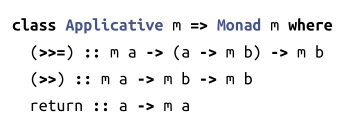
\includegraphics[width = 6 cm]{./images/monad.png} 

{\fontfamily{lmtt}\selectfont (>>=): } bind

{\fontfamily{lmtt}\selectfont (>>): }  Mr.Pointy: sequencing operator.

A monad is not
\begin{itemize}
  \renewcommand\labelitemi{{\footnotesize \textcolor{blue5}{$\blacksquare$}} }
  \item Impure. 

    {\fontfamily{cmtt}\selectfont IO} is an abstract datatype that allows impure, effectful, actions and it has {\fontfamily{cmtt}\selectfont Monad} instance.
  \item Imperative programming language. While used  for \textit{sequencing actions} that looks like imperative ones, there are commutative monads that do not order actions. ({\fontfamily{cmtt}\selectfont Reader})
  \item About strictness.

    The monadic operations of {\fontfamily{cmtt}\selectfont bind} and {\fontfamily{cmtt}\selectfont return} are nonstrict. Some operations can be made strict within a specific instance.

\end{itemize}
Not require math, category theory.

\subsection*{{\fontfamily{lmss}\selectfont \underline{Do syntax and Monad}}}  
We can evaluate {\fontfamily{cmtt}\selectfont IO} actions multiple times.

  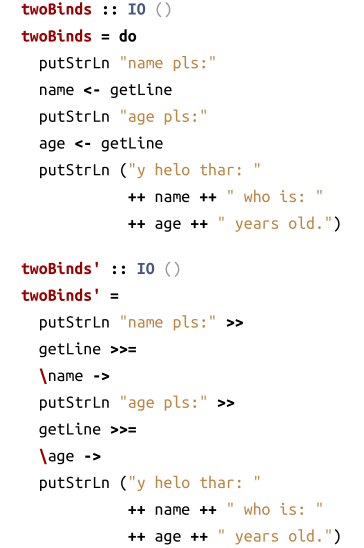
\includegraphics[width = 7 cm]{./images/dosyntax.png} 

  \subsection*{{\fontfamily{lmss}\selectfont \underline{Maybe Monad}}}
    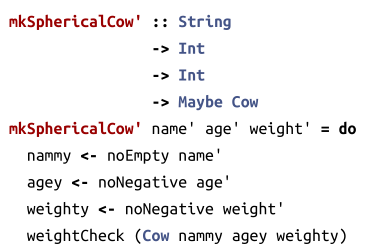
\includegraphics[width = 6 cm]{./images/mkCow.png} 
  
  Why can't we do this with {\fontfamily{cmtt}\selectfont Applicative}? Because our {\fontfamily{cmtt}\selectfont weightCheck} function depends on the prior existence of a {\fontfamily{cmtt}\selectfont Cow} value and returns more monadic structure in its return type {\fontfamily{cmtt}\selectfont Maybe Cow}.
\begin{itemize}
  \renewcommand\labelitemi{{\footnotesize \textcolor{blue5}{$\blacksquare$}} }
  \item With the {\fontfamily{cmtt}\selectfont Maybe Applicative}, each {\fontfamily{cmtt}\selectfont Maybe} computation fails or succeeds independently of each other. We are lifting functions that are also {\fontfamily{cmtt}\selectfont Just} or {\fontfamily{cmtt}\selectfont Nothing} over {\fontfamily{cmtt}\selectfont Maybe} values.
  \item With the {\fontfamily{cmtt}\selectfont Maybe Monad}, computations contributing to the final result can choose to return {\fontfamily{cmtt}\selectfont Nothing} based on previous computations.
\end{itemize}

When it fails: {\fontfamily{cmtt}\selectfont Nothing >>= $\_ \quad$ = Nothing}, the {\fontfamily{cmtt}\selectfont bind} function will leave the entire rest of the computation produce a {\fontfamily{cmtt}\selectfont Nothing} value.\\    
  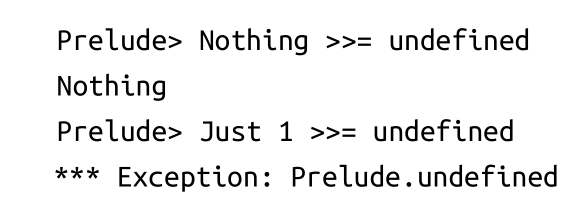
\includegraphics[width = 6 cm]{./images/bindundefined.png} 

  \subsection*{{\fontfamily{lmss}\selectfont \underline{Either Monad}}}
  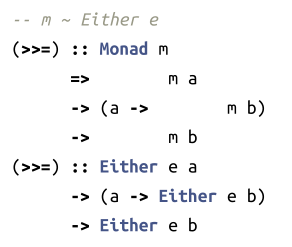
\includegraphics[width = 4.5 cm]{./images/eithermonad.png} 
 
  The problem is that we can't make a {\fontfamily{cmtt}\selectfont Monad} instance for {\fontfamily{cmtt}\selectfont Validation} that accumulates the errors like the Applicative does. Instead, it would be identical to {\fontfamily{cmtt}\selectfont Either}'s one.

  \section{Monad laws}
\begin{itemize}
  \renewcommand\labelitemi{{\footnotesize \textcolor{blue5}{$\blacksquare$}} }
  \item \textbf{\textcolor{blue5}{\fontfamily{lmss}\selectfont Identity laws.}} 
    {\fontfamily{cmtt}\selectfont return} should be neutral and not perform any computation.

      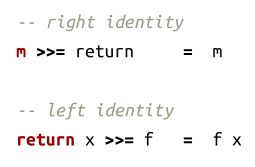
\includegraphics[width = 3.7 cm]{./images/identity.png} 

  \item \textbf{\textcolor{blue5}{\fontfamily{lmss}\selectfont Associativity.}}

      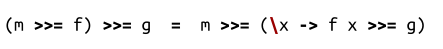
\includegraphics[width = 6.3 cm]{./images/associativity.png} 

      Regrouping the functions should not have any impacts on the final result, same as the associativity of {\fontfamily{cmtt}\selectfont Monoid}.
    
\end{itemize}   

\section{Definition}
\begin{Def}[Monad]
  Functorially applying a function which produces more structure and using {\fontfamily{cmtt}\selectfont join} to reduce the nested structure.
\end{Def}

A \textit{monadic function} is one which generates more structure after having been lifted over monadic structure.\\
  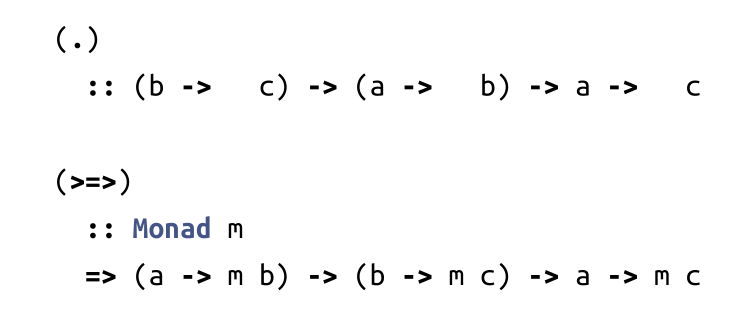
\includegraphics[width = 6 cm]{./composition.png} 

  \textit{bind} is {\fontfamily{cmtt}\selectfont >>=} 


\end{document}
